\documentclass{IEEEtran}
\usepackage[utf8]{inputenc}
\usepackage[alsoload=synchem,load=named]{siunitx}
\usepackage[version=4]{mhchem}
\usepackage{amsmath}
\usepackage{graphicx}
\usepackage[citestyle=ieee,sorting=none,bibencoding=utf8,backend=biber]{biblatex}

\graphicspath{{images/}}
\bibliography{bib}

\let\DeclareUSUnit\DeclareSIUnit
\let\US\SI
\DeclareUSUnit\foot{ft}
\DeclareUSUnit\inch{in}

\author{Powers-Luhn, J.R.}
\title{A Review of Methods for Enrichment Measurement in a Gas Centrifuge Plant}
\date{May 1st, 2017}

\begin{document}
\maketitle

\begin{abstract}
Measurement of uranium enrichment is a necessary precondition to the production of nuclear fuel while simultaneously satisfying the international community as to the peaceful nature of a nuclear program. A number of mechanisms exist for measuring the enrichment of uranium when in its solid, metallic form, but the ability to measure samples during or soon after the enrichment process is desirable. This paper reviews some of the measurement techniques that may be applied at different stages of the enrichment process, as well as the results of testing and the constraints of the tests applied.
\end{abstract}

\section{Introduction}
The use of nuclear power as a replacement for carbon-emitting sources has proven attractive to several nations around the world. Most proven nuclear power plant designs require enriched uranium to use as fuel, whether produced domestically by the country involved or purchased on the international market. The need for nuclear enrichment is projected to rise 21\% of its 2015 levels by 2020, while the world capacity is expected to exceed requirements by 16\% in that same year \cite{worldnuclear}. This naturally raises the question of how to convince other nations that this enrichment is intended for peaceful use and not in the production of undeclared nuclear weapons.

Several methods exist for measuring the enrichment of uranium in its solid or metallic forms. Many of these use spectral analysis, either of a broad range of energies or comparing a purely $\ce{^{235}U}$ emission (\SI{186}{\kilo\electronvolt}) to a background value or one proportional to the amount of total uranium. This technique requires calibration using two samples in containers with similar wall thicknesses that are sufficiently thick themselves (on the order of 8 mean free paths). Other techniques allow for self-calibration using a known $\ce{^{235}U}$ spectrum and a $\ce{^{238}U}$ spectrum. These spectra are similar enough (see figure \ref{fig:hpgespectra}) to require high resolution, high-purity germanium (HPGe) detectors \cite{Dragnev1977}. This is less useful for measuring the enrichment of gaseous uranium compounds used in gas-centrifuge enrichment plants, as it would require the piping through which the uranium flows to be greater than \SI{1}{\meter} in diameter \cite{tape}.

Measurement of uranium enrichment in industrial environments introduces several complications, categorized in table \ref{tab:unknowns}. Pressure and temperature of the \ce{UF_6} gas are combined into a density or total uranium measurement. The presence of wall deposits complicates the measurement of the gas in the piping system, as each produce the \SI{186}{\kilo\electronvolt} gamma characteristic of \ce{^{235}U}. Additionally, these wall deposits contain other isotopes, including \ce{^{234}Th}, which produces both \SI{\approx 92}{\kilo\electronvolt} gammas (interfering with \ce{UF_6} fluorescence) and a \SI{184.8}{\kilo\electronvolt} gamma (interfering with direct measurement of the \ce{^{235}U} signal). 

An ideal enrichment measurement system should have the following properties:

\begin{itemize}
	\item Automated: the need for human interference to record measurements is undesirable. The introduction of external inspectors into a nuclear facility is a matter of negotiation with the host nation, for reasons both innocent (protection of proprietary information, potentially pertaining to national security) and nefarious (the illicit production of weapons).
	\item Representative: measurements taken should represent the final product of the enrichment chain. The ideal location for sampling should be at the point where the transport and storage cylinders are filled. Multiple fill stations would require multiple sampling apparati. Alternatively, measurement of the storage and transport cylinders should be complete or at least representative. If the sampling method is predictable it is possible for a malicious actor to bypass the sampling process and divert material thereby.
\end{itemize}

\begin{center}
\begin{centering}
\begin{table}
	\centering
	\caption{Unknown values in enrichment measurement\label{tab:unknowns}}
	\begin{tabular}{c c}
		\hline
		Environment & Background \\
		& Power supply \\
		\hline
		Gas Properties & Pressure \\
		& Temperature \\
		& Mass flow rate \\
		& \textbf{Enrichment} \\
		\hline
		Piping & Thickness \\
		& Material \\
		\hline
		Wall Deposits & Thickness \\
		& Age \\
		& Composition \\
		\hline
	\end{tabular}
\end{table}
\end{centering}
\end{center}

\begin{centering}
\begin{figure}
\centering
\begin{center}
	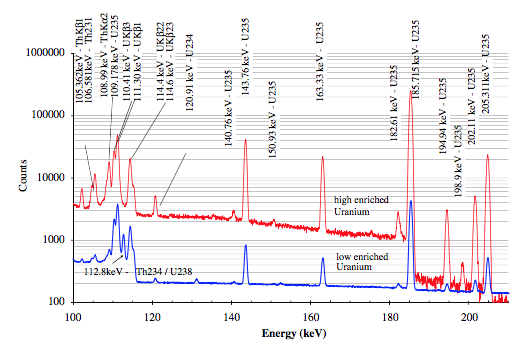
\includegraphics[width=0.4\textwidth]{hpgespectra}
	\caption{Spectra for HEU and LEU for $\ce{UF_6}$ and HPGe detector \cite{RN59}\label{fig:hpgespectra}}
\end{center}
\end{figure}
\end{centering}

\section{Stages for enrichment measurement}

\subsection{Gas phase}
Enrichment can be measured in the gas phase of $\ce{UF_6}$ for a typical gas centrifuge plant. This technique, however, faces a number of challenges. The traditional enrichment meter principle is not applicable here, as the mean free path for the pressures in question (on order of \SI{50}{\torr}) is approximately \SI{50}{\meter} \cite{RN59}. Also, number of variables occur in as-built enrichment plants. First, any calculation of enrichment requires knowledge of both the $\ce{^{235}U}$ content in the gas and the total amount of uranium. It requires correction for the detector geometry, but also for the total gaseous content in the section of the enrichment pipe being measured.

A series of tests were performed at Oak Ridge National Laboratory to determine the validity of enrichment measurement in gaseous $\ce{UF_6}$ samples using the \SI{186}{\kilo\electronvolt} peak \cite{OLEMtest}. These tests examined a variety of gas pressures at a number of different enrichment values \SIlist{0.71;2.97;6.0;93.7}{\percent}. Five different algorithms to calculate the signal produced by the $\ce{^{235}U}$ were employed and evaluated, with each calibrated to the same \SI{4.62}{\percent} sample. The first measured the area under the \SI{186}{\kilo\electronvolt} peak with a trapezoidal background region removed. Next, algorithms 1 and 2 attempted to improve the Poisson statistics by taking the total area under the \SI{186}{\kilo\electronvolt} peak and the \SI{143}{\kilo\electronvolt} and \SI{186}{\kilo\electronvolt} peaks respectively. The next examined the area under the \SI{143}{\kilo\electronvolt} and \SI{186}{\kilo\electronvolt} peaks with a user-supplied background removed. Finally, they employed an adaptive background subtraction method, as shown in figure \ref{fig:adaptivebackground}. No one method drastically outperformed any of the others, though they provide recommendations for the best algorithm to use as a function of region of interest and stated enrichment value.

\begin{centering}
\begin{figure}
\begin{center}
	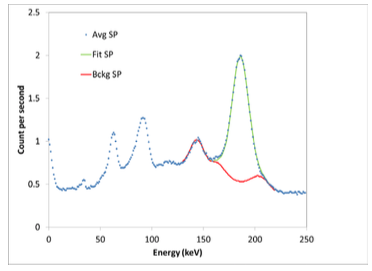
\includegraphics[width=0.4\textwidth]{adaptivebackground}
	\caption{Adaptive background subtraction for \SI{186}{\kilo\electronvolt} peak \cite{OLEMtest}\label{fig:adaptivebackground}}
\end{center}
\end{figure}
\end{centering}

Methods for correcting for the presence of uranium and thorium wall deposits have been investigated. Using two detectors that present different solid angles, it is possible to discount the influence of the wall deposits and thereby only measure the gas \cite{RN59}. This method has been verified via monte carlo and analytical methods to work for a variety of geometries, including a single detector that can be rotated to take measurements from two different angles \cite{RN43,RN56}. In this method, a collimator is selected such that it primarily examines the piping (and therefore the uranium and other isotopes deposited on the piping). After a reasonable counting time (on order of tens of minutes), the detector is rotated to present a larger solid angle to the gas piping system. An illustration of a two-detectors setup is shown in figure \ref{fig:twogeometry}. 

Determining the total $\ce{UF_6}$ content in a section of pipe can be achieved via a flourescence measurement produced by a $\ce{^{109}Cd}$ x-ray source. $\ce{^{109}Cd}$, however, has a half life of only \SI{461}{\day}, meaning that the rate at which it should be replaced is disagreeably high. Ianakiev, et al, studied the viability of replacing the $\ce{^{109}Cd}$ source with an x-ray tube and a silver or ruthenium notch filter \cite{RN64}. Consistent results (\num{\pm0.5}\% enrichment) were obtained for a range of gas pressures from \SIrange{5}{70}{\torr}. While this was not experimentally verified in the presence of wall deposits, similar geometric techniques to those described for the $\ce{^{109}Cd}$ should perform as well for this source.

Active measurement of gaseous enrichment has been studied. $\ce{^{235}UF_6}$ and $\ce{^{238}UF_6}$ show slight differences in their spectra in the infrared region, as shown in figure \ref{fig:tlds}. Analysis of the transmittance of several energies of interest shows accurate measurements across a range of enrichment values \cite{RN66,RN67}. Deploying this method to existing plants is nontrivial, however, as it requires a window that is both transparent to the frequencies of interest and resistant to the chemical effects of \ce{UF_6}, which produces \ce{HF} in the presence of water vapor. \ce{BF_3} is a suitable window material, but this means that specialized sections of pipe must be inserted into the enrichment process. Measurements have yet to be taken under conditions that have allowed for the presence of significant wall deposits, and this measurement remains sensitive to the density of \ce{UF_6} in the piping.

\begin{centering}
\begin{figure}
\begin{center}
	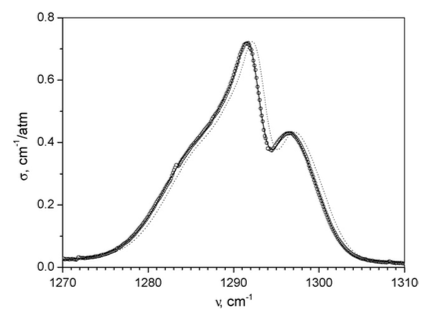
\includegraphics[width=0.4\textwidth]{tlds}
	\caption{Absorption of infrared light in the vicinity of \SI{1290}{\per\centi\meter} by \ce{^{235}UF_6} vs. \ce{^{238}UF_6} \cite{RN66}\label{fig:tlds}}
\end{center}
\end{figure}
\end{centering}

\begin{centering}
\begin{figure}
\begin{center}
	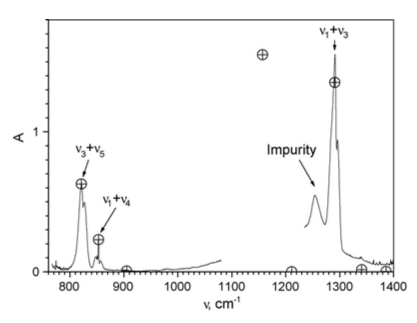
\includegraphics[width=0.4\textwidth]{tlds2}
	\caption{Absorption spectra for \ce{UF_6} in the infrared range \cite{RN66}\label{fig:tlds2}}
\end{center}
\end{figure}
\end{centering}

Imaging techniques also show promise for the determination of enrichment, especially in the verification of design information (e.g., which portions of piping are in use) in enrichment plants. Burks, et al \cite{RN47}, were able to use a Compton scattering-based imager to detect a small (\SI{2.5}{\gram}) $\ce{^{235}U}$ source in the presence of a much larger (\SI{400}{\gram}) sample of depleted uranium. These image was taken at an assortment of distances (\SIrange{4}{9}{\foot}), with the HEU clearly visible up to \SI{6}{\foot}. This method worked best as a verification tool, and suffered from a poor point spread function at energies of interest (\SI{186}{\kilo\electronvolt}). It was also comparatively insensitive to low-enriched uranium samples and very sensitive to holdup in the piping material. It might therefore provide a good mechanism for periodic inspection while not meeting the criteria for continuous monitoring of enrichment plants.

\begin{centering}
\begin{figure}
\begin{center}
	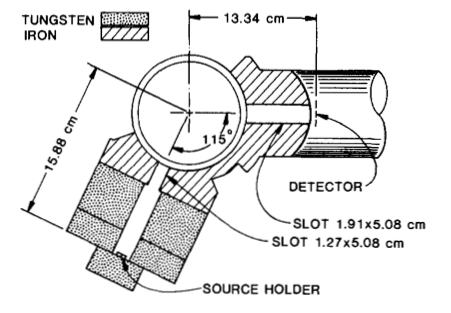
\includegraphics[width=0.4\textwidth]{twogeometry}
	\caption{Two-geometry method for correcting for wall deposits of \ce{UO_2F_2} \cite{RN59}\label{fig:twogeometry}}
\end{center}
\end{figure}
\end{centering}

\subsection{In transit/storage cylinders}
Both before and after enrichment, the $\ce{UF_6}$ is stored and transported in the form of cylinders, typically of model 30B (\SI{30}{\inch} by \SI{6}{\foot}; commonly used for storage of UF6 in product cylinder bays) and larger model 48B cylinders (\SI{48}{\inch} by \SI{12}{\foot}). Measurement at this point has the advantage of higher density and a standardized container configuration, allowing for total uranium content to be measured via simple weight methods. The amount of $\ce{^{235}U}$ present can then be measured using the strength of the \SI{186}{\kilo\electronvolt} gamma emission. This method leaves something to be desired, however, as

\begin{enumerate}
\item the distribution of $\ce{UF_6}$ may not be uniform within the cylinder: depending on the cylinder's attitude, temperature, and fill pressure at the time the cylinder was filled, asymmetries in either the axial, radial or both dimensions are expected (as in figure \ref{fig:cylinderdeposition}, and
\item the density of the material in the cylinder is dependent on the filling method and filling conditions, resulting in potential self-shielding.
\end{enumerate}

\begin{centering}
\begin{figure}
\begin{center}
	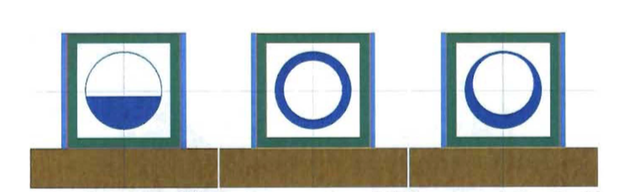
\includegraphics[width=0.4\textwidth]{cylinderdeposition}
	\caption{Asymmetric deposition of solidified \ce{UF_6} in transport and storage cylinders \cite{RN63}\label{fig:cylinderdeposition}}
\end{center}
\end{figure}
\end{centering}

Other means of measuring the \ce{^{235}U} content of transport cylinders have been investigated. One such mechanism involves measuring the neutrons produced by the spontaneous fission and ($\alpha$,n) reactions of the uranium in the cylinder \cite{RN58,RN63}. This technique uses coincidence counting to differentiate between spontaneous fission neutrons (dominated by \ce{^{238}U}) and neutrons produced by ($\alpha$,n) reactions. The ratio of these events gives the relative fraction of \ce{^{234}U}, which is proportional to \ce{^{235}U}. This holds true for samples less than a few \si{\kilo\gram}; in larger samples, fission multiplication dominates the doubles signal, meaning that \ce{^{235}U} contributes directly \cite{RN63}.

In an attempt to compensate for the low resolution of \ce{NaI(Tl)} detectors for enrichment measurement in cylinders, the suitability of lanthanum bromide detectors was investigated \cite{RN60}. Unfortunately, it was determined that the tradeoffs it presented (lower resolution than HPGe; lower efficiency than \ce{NaI(Tl)}) meant that it was at best comparable to these better-characterized detectors; at worst (in the case of 48Y cylinders) much worse due to lower counting efficiencies.

It is of note that, while the cylinders used to store and transport $\ce{UF_6}$ are essentially standardized, construction tolerances of \SI{\pm 0.5}{\milli\meter} lead to uncertainty in enrichment measurement of $\pm$5\% \cite{RN58}.

Promising work has been started at PNNL to produce the desired automated measurement of enrichment in \ce{UF_6} cylinders. \ce{NaI(Tl)} and \ce{LaBr_3} detectors were used to measure gamma rays produced by the reaction \ce{^{19}F(\alpha,n)\rightarrow^{56}Fe(n,\gamma)}. These high energy gamma rays should be proportional to the alpha decay of \ce{^{238}U} and can be combined with measurements of the \SI{186}{\kilo\electronvolt} gamma from \ce{^{235}U} to produce enrichment measurements \cite{RN57,zalavadia2015hybrid}. Work on this system is ongoing as of 2016.

\subsection{Forensic}
It is sometimes of interest to track the use of enrichment facilities after their active use. This can provide forensic information useful in informing policy makers as to the capabilities of nations and groups in the past. 

One proposed method uses the long biological residence times of various nuclides and chemicals used in the processing of nuclear material \cite{RN45}. Samples are taken from these plants and animals and analyzed using NMR techniques. This process is illustrated in figure \ref{fig:bioassay}. Test studies indicate that these samples survive analysis and show variation to indicate industrial proceses, but this technique is limited in that it depends on a well-understood background of other industrial work that might involve these chemicals but not represent nuclear processing or enrichment.

\begin{centering}
\begin{figure}[h]
\begin{center}
	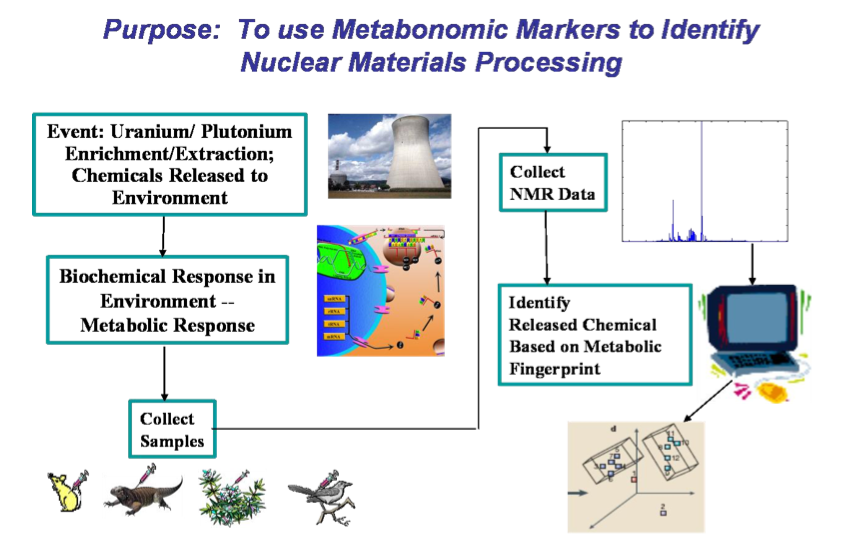
\includegraphics[width=0.4\textwidth]{bioassay}
	\caption{Nuclear forensics by biological buildup \cite{RN45}\label{fig:bioassay}}
\end{center}
\end{figure}
\end{centering}

\section{Conclusions}
A number of experimental techniques for measuring or verifying the enrichment of \ce{UF_6} are available and suitable for use in enrichment plants. Many of these meet the criteria stated above--they can be automated so as not to require the presence of inspectors, and they represent the potential for 100\% sampling of the product of an enrichment plant. Continued development of detectors to measure both centrifuge plant piping and transport/storage cylinders should yield more commercially viable form factors. Testing at a variety of as-built plants is appropriate to determine how feasible each design is and to check the produced values against known samples in industrial environments.

%\nocite{*}
\printbibliography

\end{document}